\documentclass[journal,a4paper,twoside]{sty/IEEEtran}

\usepackage[utf8]{inputenc}
\usepackage[slovene]{babel}
\usepackage[T1]{fontenc}
\usepackage{sty/EVrevija}
\usepackage{graphicx}
\usepackage{tikz}
\usepackage[affil-it]{authblk}

\begin{document}

% naslov prispevka, lahko uporabite en linebreak \\
\title{Regulacija asinhronskega motorja v slabljenju polja}

\authors{Mitja Ali"c} 
\address{E-pošta: mitja1357@gmail.com}

\abstract{}

\keywords{dvoosni koordinatni sistem, magnetilni tok}

% Priimki avtorjev in kratek naslov članka za tekočo glavo
\markboth{Ali"c}{Regulacija asinhronskega motorja v slabljenju polja}

% make the title area
\maketitle

% Naslov in kratek povzetek v angleščini
\english{Control of asynchronous motor in the field weakening}
{Mitja in english here please.}

\section{Uvod}

Kot "student fakultete za elektrotehniko na Univerzi v Ljubljani sem pri predmetu Integrirani pogonski sistemi delal na regulaciji pogona v nadnazivni hitrosti. V nadnazivnih hitrostih pogon za"cne omejevati napetostna zmo"znost napajalnega pretvornika.  Ponavadi se poslu"zimo zmanj"sevanje referen"cne vrednosti amplitude magnetnega sklepa v zra"cni rezi v obratnem razmerju s vrtilno hitrostjo. To pa nam ne zagotovi maksimalnega navora. S programskim paketom Matlab sem simuliral delovanje motorja v nadnazivnih hitrostih in pri tem preizkusil razli"cne metode.

\section{Standardna metoda}
Frekven"cni pretvornik pogona ima definirano napetostno in tokovno limito. Napetostna limita je odvisna od enosmerne napetosti generirane v pretvorniku.
Zaradi omejene izhodne napetosti pretvornika je lahko maksimalna napetost:
\begin{equation}
u_{Sd}^2+u_{Sq}^2= U_{dc}^2
\label{eq:napetost1}
\end{equation}

$u_{Sd}$ in $u_{Sq}$ predstavljata vzol"zno in pre"cno komponento  napetosti v dvoosnem koordinatnem sistemu \cite{servopogoni}. Napetosti sta odvisni od pre"cne, vzdol"zne komponente toka in magnetilnega  toka (ena"cbi \ref{eq:usd}, \ref{eq:usq}). Magnetilna komponenta toka je odvisna le od vzdol"zne komponente toka (ena"cba \ref{eq:imr}).

\begin{equation}
u_{Sd}= R_S i_{Sd}+L_s' \frac{di_{Sd}}{dt}- L_s' \omega_{mr} i_{Sq}+(L_s-L_s')\frac{di_{mr}}{dt}
\label{eq:usd}
\end{equation}
\begin{equation}
u_{Sq}= R_s i_{Sq}+L_s' \frac{di_{Sq}}{dt} + L_s' \omega_{mr}i_{Sd}+(L_s-L_s')\omega_{mr}i_{mr}
\label{eq:usq}
\end{equation}

%\begin{equation}
%T_R\frac{di_{mr}}{dt}+i_{mr} =i_{Sd}
%\label{eq:imr}
%\end{equation}


V stacionarnem stanju so vrednosti odvodov enaki 0. Magnetilni tok ima enako vrednost kot $i_{sd}$. Pri vi"sjih vrtilnih hitrostih postane ohmski padec napetosti zanemarljiv in ena"cbi se poenostaviti:

\begin{equation}
u_{Sd}= - L_s' \omega_{mr} i_{Sq}
\label{eq:usd_stat_w}
\end{equation}
\begin{equation}
u_{Sq}= - L_s \omega_{mr}i_{Sd}
\label{eq:usq_stat_w}
\end{equation}
 Ena"cbi \ref{eq:usd_stat_w} in \ref{eq:usq_stat_w} vstavimo v \ref{eq:napetost1}:

\begin{equation}
(L_s' \omega_{mr} i_{Sq})^2+(L_s \omega_{mr}i_{Sd})^2= U_{dc}^2
\label{eq:napetostnalim1}
\end{equation}

Rezultat predstavlja maksimalno vrednost statorskih tokov v dvoosnem koordinatnem sistemu, v odvistnosti od napetosti. "Ce izraz predelamo dobimo ena"cbo iz katere prepoznamo elipso: 

\begin{equation}
(\frac{i_{Sd}}{a})^2+(\frac{i_{Sq}}{b})^2 = 1
\label{eq:napetostnalim}
\end{equation}
$a$ in $b$ predstavljata pol osi elipse, $a=U_{dc}/(\omega_{mr}L_s)$, $b=U_{dc}/(\omega_{mr}L_s')$. Polosi sta funkciji vrtilne hitrosti in z nara"s"canjem hitrosti postajati manj"si.

Vsak motor je konstruiran za dolo"cene pogoje in temu primerno je dolo"cen tudi nazivni tok. "Ce stroj obratuje z vi"sjim tokom kot je nazivni se bo zaradi toplotnih izgub v navitjih za"cel segrevati. S segrevanjem pa lahko deformiramo stroj ali mu s takim obratovanjem skraj"samo "zivljensko dobo. Maksimalen tok v motor je tako:

\begin{equation}
i_{Sd}^2+i_{Sq}^2=\hat{I}_{n}^2
\label{eq:tokovnalim}
\end{equation}

Pogojema dolo"cenima z ena"cbama \ref{eq:napetostnalim} in \ref{eq:tokovnalim}, mora statorski tok vedno ustrezati. Ob takem obratovanju bo stroj lahko deloval celotno "zivljensko dobo.



"Ce grafi"cno ponazorimo napetostno in tokovno limito nam presek mej teh limit prikazuje to"cko, ki ozna"cuje najve"cjo vrednost tokovnega vektorja (Slika \ref{fig:napetostna_tokovna_limita_slika}). V tej to"cki motor ustvari najve"cji navor Tokovna limito predstavlja kro"znica, ki je neodvisna od hitrosti. Elipsa predstavlja napetostno limito, ki je odvisna od hitrosti. Pri ni"zjih vrtilnih hitrostih sta polosi ve"cji od polmera tokovne limite(Napetostna limita za $\omega_1$ na sliki \ref{fig:napetostna_tokovna_limita_slika}), zato vpliva na tokovni vektor le tokovna limita (tokovni vektor se mora gibati znotraj zelenega kroga). Pri vi"sjih vrtilnih hitrostih se polosi elipse zmanj"sati in tokovni vektor se mora prilagoditi tudi napetostni limiti(Napetostna limita za $\omega_2$ na sliki \ref{fig:napetostna_tokovna_limita_slika}). Gibati se mora po preseku obmo"cja ki ga ozna"cujet obarvan del.

\begin{figure}
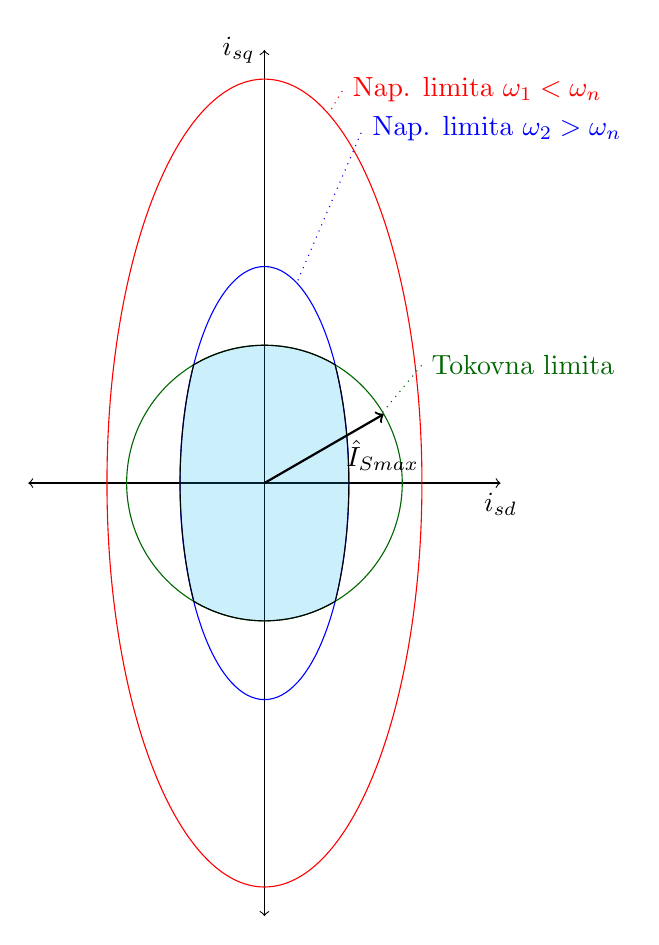
\begin{tikzpicture}[scale=0.5]
%koordinatni sistem
\draw [<->](-6,0)--(6,0) node[anchor=north]{$i_{sd}$};
\draw [<->](0,-11)--(0,11) node[anchor=east]{$i_{sq}$};

%elipsa za nizke hitrosti
\draw [red](0,0)ellipse  (4 and 10.26);
\draw [dotted,red] (1.7,9.5)--(2,10) node[anchor=west]{Nap. limita $\omega_1 < \omega_n $};

%elipsa za visoke hitrosti
\draw [dotted,blue] (0.85,5.15)--(2.5,9) node[anchor= west]{Nap. limita $\omega_2 > \omega_n$};
\draw [blue] (0,0)ellipse (2.145 and 5.5);

%tokovna limita in oznacba
\draw [black!60!green](0,0)circle (3.5); 
\draw [dotted,black!60!green] (3,1.8)--(4,3) node[anchor= west]{Tokovna limita};

    \fill[cyan,draw=black, fill opacity=0.2] (1.79693,-3.0035) arc (-33:33.1:2.145 and 5.5)--(1.79693,3.0035)arc(59.1:180-59.1:3.5)--(-1.79693,3.0035) arc (180-33:180+33:2.145 and 5.5)--(-1.79693,-3.0035)arc(180+59.1:360-59.1:3.5);
    
\draw[->, thick](0,0)--(3.03,1.75);
\draw (3,0.7) node{$\hat{I}_{Smax}$};

\end{tikzpicture}
\caption{Prikaz napetostne in tokovne limite pri dveh vrtilnih hirostih}
\label{fig:napetostna_tokovna_limita_slika}

\end{figure}


Pri vrtilnih hitrostih vi"sjih od nazivne se standardno uporablja slabljenje polja po prvi potenci. Pri tej metodi zni"zujemo vrednost magnetilnega toka v obratnem razmerju z vrtilno hitrostjo,
\begin{equation}
\label{eq:standardna_metoda}
i_{mag}^*=i_{magn}\frac{\omega_n}{\omega_r}
\end{equation}

kjer $i_{magn}$ predstavlja nazivno vrednost magnetilnega toka, $\omega_{n}$ predstavlja nazivno vrtilno hitrost in $\omega_{r}$ trenutno vrtilno hitrost rotorja. Ulomek $\frac{\omega_r}{\omega_n}$ bi lahko nadomestili tudi z vrtilno hitrostjo v p.u. sistemu. Maksimalna vrednost pre"cne komponente toka pri tej metodi dolo"ci ena"cba \ref{eq:tokovnalim}:

\begin{equation}
i_{sqmax}=\sqrt{\hat{I}_n^2-i_{sd}^{*2}}
\label{maxqtok}
\end{equation}.










\section{Izbolj"sana metoda}



V nadeljevanju sta opisani dve metodi nastavljanja "zeljene vrednosti magnetilnega toka, pri katerih je magnetna nasi"cenost zanemarjena. Prva metoda ustvari ve"cji navor v obmo"cju nad vrtilno hitrostjo. Druga metoda temelji na prvi metodi, vendar lahko ob prehodnih pojavih ustvari ve"cji navor kot prva tehnika tehnika.

\subsection{Prva izbolj"sana metoda}



Ob definiranem frekven"cnem pretvorniku nam ta poda makismalno vrednost izhodne napetosti in toka. Ob upo"stevanju ena"cb \ref{eq:napetostnalim}, \ref{eq:standardna_metoda} in \ref{maxqtok} lahko izrazimo vrtilno hitrost pri kateri je "se lahko nazivni magnetilni tok. Vrtilna hitrost pri kateri se poslu"zimo tehnike slabljenja polja je odvisna od parametrov frekven"cnega pretvornika, nazivnega magnetilnega toka ter statorske in stresane induktivnosti. 

\begin{equation}
\omega_n=\frac{\hat{U}_{smax}}{\sqrt{i_{sdn}^{*2}(L_s^2-L_s'^2)+(L_s'\hat{I}_n)^2}}
\label{nazivnaw}
\end{equation}



V podro"cju slabljenja polja bo navor bolj"siod standardne metode ob upo"stevanju limit ki jih dolo"cati ena"cbi \ref{eq:napetostnalim1} in \ref{eq:tokovnalim}. 

\begin{equation}
\label{eq:zeljentok1}
i_{sd}^*=\sqrt{\frac{(\frac{\hat{U}_{dc}}{\omega})^2-(L_s'\hat{I}_{smax})^2}{L_s^2-L_s'^2}}
\end{equation}

Vrednost "zeljene vrednosti magnetilnega toka in pre"cne komponente toka glede na vrtilno hitrost v podro"cju slabljenja polja lahko razberemo iz slike \ref{fig:napetostna_tokovna_limita_slika}, v prese"ci"s"cu elipse in kro"znice. 














\subsection{Druga izbolj"sana metoda}


Pri prvi metodi smo upo"stevali da je motor v stacionarnem stanju in mangetilni tok je enak vzdol"zni komponenti toka.
Navorno ena"cbo za asinhroski motor lahko zapi"semo tudi kot:
\begin{equation}
\label{eq:navor2}
M_{el}=\frac{3}{2}p_p \frac{L_m}{L_r}|\psi_{rd}|i_{Sq}
\end{equation}
 pri "C
cemer je $\psi_{r}$ predstavlja rotorski magnetni sklep. Le ta je odvisen od magnetilnega toka, ki je posledica vzdol"zne komponente statorskega toka.
\begin{equation}
\label{eq:flux}
\psi_{rd}= \frac{L_m i_{Sd}}{1+T_r p}
\end{equation}

kjer $p$ predstavlja operator odvajanja po "casu $p=d/dt$ in $T_r$ rotorska "casovna konstanta.

Re"sitev ena"cebe \ref{eq:flux} lahko zapisemo kot:
\begin{equation}
\label{eq:Lm+delta}
\psi_{rd}=L_m i_{Sd}+\Delta \psi_{rd}
\end{equation}
 kjer je
 
 \begin{equation}
\label{eq:delta}
\Delta \psi_{rd}=(\psi_{rd}(t_0)-L_m i_{Sd}(t_0))e^{\frac{t_0-t}{T_r}}
\end{equation}

$t_0$ predstavlja za"cetni "cas. Elektromagnetni navor je tako povi"san
\begin{equation}
\label{navor3}
M_{el}=\frac{3}{2}p_p \frac{L_m}{L_r}(L_m i_{Sd}+\Delta \psi_{rd})i_{Sq}
\end{equation}

Ob upo"stevanju neenakosti magnetilnega toka in vzdol"zne komponente statroskega toka v ena"cbi \ref{eq:usq} in posledi"cno tudi v ena"cbi \ref{eq:napetostnalim}, lahko definiramo novo "zeljeno vrednost vzdol"zne komponente toka.
\begin{equation}
\label{eq:zeljentok2}
i_{Sd}^*=\frac{\sqrt{(c L_s)^2+(L_s^2-L_s'^2)[(\frac{U_{dc}}{\omega})^2-L_s'^2I_{smax}^2-c^2]}-cL_s}{L_s^2-L_s'^2}
\end{equation}
\begin{equation}
i_{sqmax}=\sqrt{\hat{I}_n^2-i_{sd}^{*2}}
\end{equation}
Pri "cemer
$$c=\frac{L_m}{L_r}(\psi_{r}(t_0)-L_m i_{Sd}(t_0))$$


\section{Simulacije in uporaba tehnik}
Simulacije sem izvedel s programskim paketom Matlab. 

Za model asinhronskega motorja sem si izbral naslednje podatke:
\begin{itemize}
\item{$P_n=0.5$ kW}
\item{$M_n = 2.5$ Nm}
\item{$U_n = 15$ V}	
\item{$I_{mrn} = 18.7$ A}
\item{$I_n = 28.4$ A}
\item{$n_N = 2200$ rpm}
\item{$R_s = 0.074$ $\mathrm{\Omega}$}
\item{$R_r = 0.0513$ $\mathrm{\Omega}$}
\item{$L_s = 2.596$ mH}
\item{$L_r = 2.559$ mH}
\item{$L_m = 2.4$ mH}
\item{$p_p = 1$  polov par}
\item{$J = 0.001$ kg $\mathrm{m}^2$}
\end{itemize}
Za izra"cune v simulaciji sem uporabil dvoosni koordinatni sistem v katerega sem pretvoril asinhronski motor.

Simuliran napetostni pretvornik je imel omejitve napetosti in toka prilagojene nazivnim parametrom asinhronskega motorja.
\begin{itemize}
\item{$U_{dc}=U_{max}=U_n\sqrt{2}=21,2$ V}
\item{$I_{max}=I_n\sqrt{2}=40,16$ A}
\end{itemize}



Motor sem reguliral z neposredno FOC metodo. Limite v regulaciji sem nastavil po izrazih v \ref{eq:napetostnalim1} in \ref{eq:tokovnalim}.
Osrednji del simulacij se je navezoval na dolo"canje vzdol"zne komponente toka. Za njeno dolo"canje sem uporabil izraza iz zgoraj teoreti"cno opisanih postopkov (ena"cba \ref{eq:zeljentok1},\ref{eq:zeljentok2}). V simulacijah sem preveril obe metodi in ocenil rezultate.

\section{Rezultati simulacij}



%
%
%\newpage
%
%
%
%Pri asinhroskih motrojih je magnetilni tok odvisen od pre"cne komponente toka(ena"cba \ref{eq:imr}). 
%Magnetni rotorski pretok je linearno odvisen od magnetilnega toka, ta pa je posledica vzdol"zne komponente statorskega toka.
%\begin{equation}
%\label{eq:flux}
%\psi_{rd}= \frac{L_m i_{Sd}}{1+T_r p}
%\end{equation}
%
%kjer $p$ predstavlja operator odvajanja po "casu $p=d/dt$ in $T_r$ rotorska "casovna konstanta. Navorno ena"cbo lahko zapi"semo tudi kot:
%\begin{equation}
%\label{eq:navor2}
%M_{el}=\frac{3}{2}p_p \frac{L_m}{L_r}|\psi_{r}|i_{Sq}
%\end{equation}
%Z upo"stevanjem, da je magnetilni tok posledica vzdol"zne komponente, ki jo reguliramo, med spremembo vrtilne hitrosti lahko upo"stevamo tudi ta parameter. "zeljeno vrednost vzdol"zne komponente toka lahko tako dolo"cimo po ena"bi iz \cite{vas}
%\begin{equation}
%\label{eq:zeljentok2}
%i_{Sd}^*=\frac{\sqrt{(c L_s)^2+(L_s^2-L_s'^2)[(\frac{U_{dc}}{\omega})^2-L_s'^2I_{smax}^2-c^2]}-cL_s}{L_s^2-L_s'^2}
%\end{equation}
%pri "cemer
%$$c=\frac{L_m^2}{L_r}(i_{mr}-i_{Sd})$$.
%V stacionarnem stanju sta magnetilni tok in vzdol"zna komponenta statorskega toka enaki in $c=0$. Izraz v  \ref{eq:zeljentok2} se poenostavi v izraz iz prve metode(ena"cba \ref{eq:zeljentok1})
%Elektromagnetni navor se lahko izrazi sedaj tudi:
%\begin{equation}
%\label{eq:navorzatok2}
%M_{el}=\frac{3}{2}p_p \frac{L_m}{L_s' L_r}\sqrt{(\frac{U_{dc}}{\omega})^2-(L_s i_{Sd}^*+c)^2\psi_{rd}}
%\end{equation}

%\begin{table}[!t]
%%\renewcommand{\arraystretch}{1.3}
%%\caption{Rezultati optimizacije D flip-flopa}
%%\label{results}
%%\centering
%%\begin{tabular}{l @{\hspace{-2mm}} r | r r r}
%%lastnost                                    &                   & original           & hitrost & poraba \\ \hline 
%%\multicolumn{4}{l}{\scriptsize $\uparrow$ in $\downarrow$ pomenita naraščajočo in padajočo fronto} \\
%%\end{tabular}
%%\end{table}
%%
%%V stolpcu poraba v tabeli \ref{results} so zbrani vadno uporabljena hitra lokalna optimizacijska metoda, npr. \cite{hooke}. Žal p
%%
%%%\centerline{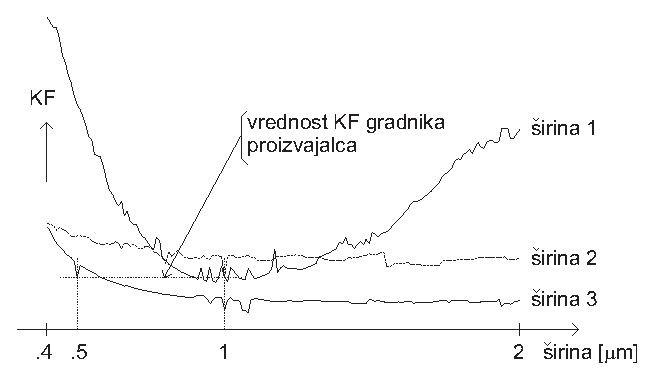
\includegraphics[width=8cm]{fig/cost_profile_slo}}



\begin{thebibliography}{10}

\bibitem[1]{servopogoni}V.~Ambro"zi"c, P.~Zajec, {\em Elektri"cni servo pogoni}, \hskip 1em plus 0.5em minus 0.4em \relax Slovensko zdru"zenje elektroenergetikov CIGR\'E-CIRED, 2016

\bibitem[2]{vas} P.~Vas, {\em Sensorless Vector and Direct Torque Control}, \hskip 1em plus 0.5em minus 0.4em \relax Oxford University Press, pp 632--641, 1998


\bibitem[3]{pogoni}R.~Fi"ser, {\em Pogonski sistemi z elektromotorji}
\end{thebibliography}







% that's all folks
\end{document}


